\newpage
\section{Sensor de temperatura}

El sensor de temperatura MAX30205 tiene una interfaz de comunicación I2C, para poder comprobar su funcionamiento de forma unitaria, fue necesario configurar la interfaz I2C con la que cuenta el dsPIC30205 y adicionalmente crear las rutinas para mantener la comunicación entre ambos componentes.\\

En la figura \ref{fig:DiagramaMAX30205} se muestra el diagrama de tiempo que describe el procedimiento que debe ser seguido para realizar la comunicación entre el MAX30205 y el dsPIC.\\


\begin{figure}[htbp!]
	\centering
	\fbox{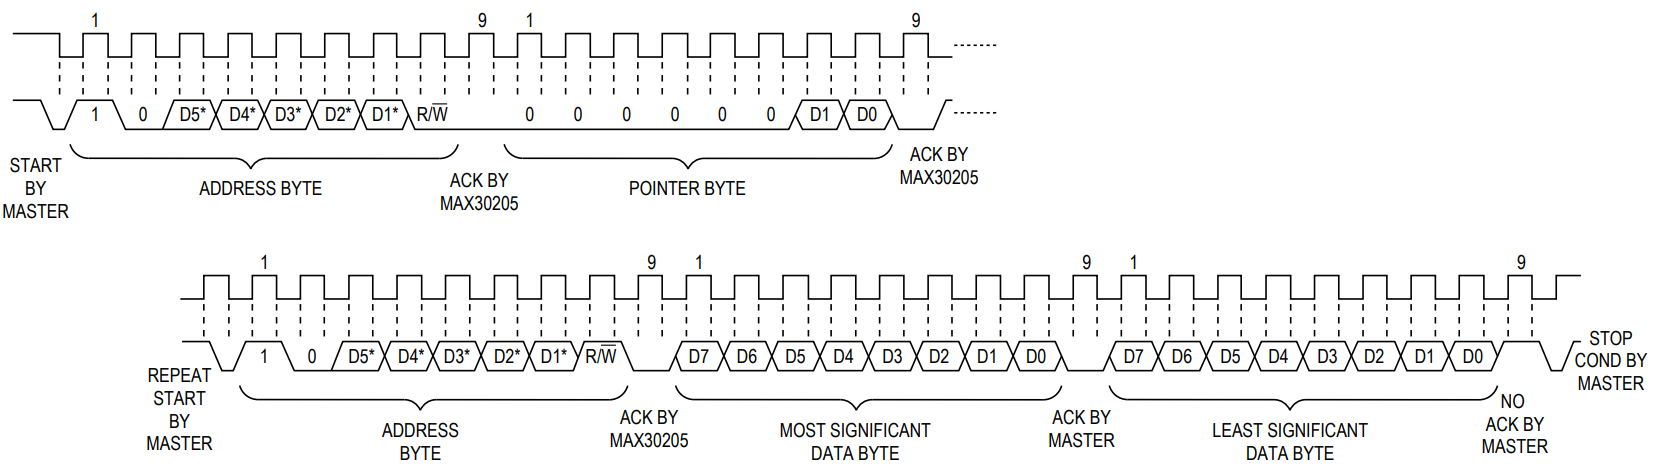
\includegraphics[width=1\textwidth]{AvancesPruebas/imagenes/diagramaI2C.png}}
	\caption{Diagrama de tiempo MAX30205.}
	\label{fig:DiagramaMAX30205}
\end{figure}

El procedimiento que se llevó a cabo para cumplir con los pasos establecidos en el diagrama de tiempo del sensor se describe a continuación.

\begin{enumerate}
	\item Se generó una condición de ''start'' para el bus I2C y de esa forma comenzar la comunicación entre ambos componentes.
	\item Se asignó una dirección al sensor a través de las terminales A0, A1 y A2. Estas terminales fueron conectadas a tierra para formar la dirección 90H, la cual fue enviada por el dsPIC al MAX30205 junto con la instrucción de escritura. Luego de ser enviada, el maestro queda a la espera de que el esclavo envíe un ACK (acknowledge) como respuesta.
	\item Para el siguiente paso se debe seleccionar el registro de temperatura (00) para indicar al sensor que únicamente se realizará la lectura de la temperatura. Al igual que en el paso anterior, el dsPIC debe esperar el ACK del sensor para continuar con la comunicación.
	\item Como se indica en el diagrama de tiempo, el maestro debe generar una condición de restart antes de seguir con el proceso de comunicación. 
	\item Una vez más el maestro debe enviar la dirección del esclavo, esta vez con la condición de lectura para comenzar a recibir las mediciones del sensor, esto no sin antes recibir el ACK del esclavo.
	\item La lectura de la temperatura se realiza en dos partes comenzando con el byte de datos más significativo que indica la parte entera de la medición y posteriormente con el byte de datos menos significativo, la cual incluye los decimales.
	\item Para terminar la comunicación, el maestro genera un NACK (no acknowledge) y por último una condición de STOP para el bus I2C.
\end{enumerate}



Para visualizar los datos recibidos del sensor, se habilitaron las terminales del UART1 y se conectó el módulo FT232 a la computadora. 
TEl resultado de la ejecución del programa con las mediciones leídas se muestra en la figura \ref{fig:ResultadoTerminalMAX30205}.\\
%
%
%\begin{figure}[htbp!]
%	\centering
%	\fbox{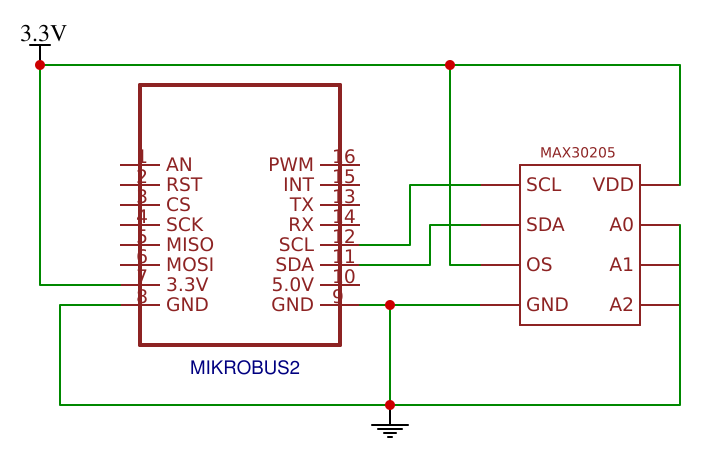
\includegraphics[width=0.7\textwidth]{AvancesPruebas/imagenes/MAX30205Conexion.png}}
%	\caption{Conexión del sensor MAX30205.}
%	\label{fig:ResultadoTerminalMAX30205}
%\end{figure}

El resultado de esta prueba muestra que el sensor de temperatura MAX30205 funciona de manera esperada y la elección realizada fue correcta.

\clearpage